\documentclass[12pt]{article}
\usepackage[margin = 1in]{geometry}
\usepackage[USenglish]{babel}
\usepackage{natbib}
\usepackage{graphicx}
\usepackage{fancyhdr}
\usepackage{setspace}
\usepackage{amsmath}
\usepackage{lscape}
\usepackage{dcolumn}
\usepackage{xcolor}
\usepackage{longtable}
\usepackage{tabularx}
\usepackage{booktabs}
\usepackage{arydshln}
\usepackage{dcolumn}
\usepackage[colorlinks=true,citecolor=red!50!black,urlcolor=blue!50!black,linkcolor=red!50!black]{hyperref}

\author{Patrick W. Kraft\footnote{Ph.D. Candidate, Stony Brook University, \href{mailto:patrick.kraft@stonybrook.edu}{patrick.kraft@stonybrook.edu}.
%A previous version of this paper was in collaboration with Laura Buchanan, Data Science NYU
}}
\date{today}

\title{Women Also Know Stuff\\
\large{Challenging the Gender Gap in Political Sophistication}\footnote{Prepared for the 75th Annual Conference of the Midwest Political Science Association, April 6-9, 2017. The manuscript and code are available on GitHub: \url{https://github.com/pwkraft/knowledge}}
}
\date{\today}

% sans serif font
\renewcommand{\familydefault}{\sfdefault}


\begin{document}
\maketitle\doublespacing\thispagestyle{empty}

\begin{abstract}\singlespacing
Studies frequently found that on average, women appear to be less informed about politics than men. However, recent research raised theoretical as well as methodological concerns regarding conventional measures of political knowledge. This paper proposes an alternative approach to assess individual political sophistication in opinion surveys. Building on theoretical frameworks that focus on the structure of political belief systems rather than factual knowledge, I examine how individuals describe their political attitudes in open-ended responses using quantitative text analysis methods. The proposed measure aims to capture the complexity of verbatim responses based on their relative length, topic diversity, and opinion diversity. Compared to traditional knowledge metrics, the new measure behaves similarly as a predictor of political attitudes and behavior and shares common determinants - with one important exception. Contrary to previous research, there is no evidence for a gender gap in political sophistication using the text-based measure. While women might score lower than men on factual knowledge about political institutions and elites, there are no differences in the complexity of expressed political attitudes. %The paper proceeds to show how the new measure can improve our understanding of gender differences in political learning as well as the consequences of political sophistication. 

\vspace{\baselineskip}
\noindent \textbf{Keywords:} political sophistication, gender gap, measurement, open-ended responses, text analysis \\

\end{abstract}
\newpage\setcounter{page}{1}


\section*{Introduction}

% REVISE: change opening to discuss gender gap first
Political sophistication is one of the most fundamental concepts in the study of political attitudes and behavior. While scholars frequently emphasized the alarmingly low levels of political knowledge among the electorate \citep{converse1964nature,carpini1996americans}, there has been a re-occurring debate about how to assess individual sophistication in the first place \citep[e.g.][]{mondak2000reconsidering,mondak2001asked,sturgis2008experiment,debell2013harder,pietryka2013analysis}. Many analyses exclusively rely on individual levels of political knowledge measured by correctness of factual knowledge questions. However, recent research points to important differences between types of knowledge questions that have previously been disregarded \citep{barabas2014question}. Furthermore, scholars argue that factual political knowledge, as measured in many surveys, may not be theoretically relevant \citep{lupia2006elitism} and does not necessarily capture how people structure their attitudes and beliefs \citep[e.g.][]{luskin1987measuring}. As such, measuring sophistication solely based on answers to political trivia may misclassify respondents who cannot recall these facts, but do indeed possess a coherent cognitive framework of political ideas.

One example for such potential misclassifications is the issue of gender differences in sophistication. On the basis of conventional factual knowledge measures, women frequently appear to be less informed about politics than men \citep{verba1997knowing,wolak2011roots}. However, some scholar suggested that these differences might be rooted in the conceptual and methodological issues related to the measurement of sophistication. For example, \citet{mondak2004knowledge} argues that at least part of the gender gap in sophistication can be attributed to the fact that women are less likely to guess than men when facing a factual knowledge question for which they do not know an immediate answer. Others suggest that the gap can be attenuated by focusing on gender-relevant political knowledge \citep[e.g.,][]{dolan2011women} or by providing policy-specific information \citep[e.g.,][]{jerit2017revisiting}. Considering the potential biases related to conventional metrics of political knowledge, is the diagnosis of a consistent gender gap in sophistication really warranted?

The present paper addresses this question by proposing an alternative measure of political sophistication based on the the complexity of open-ended survey responses. As such, inferences about the respondents' level of political sophistication are based on how they describe their preferences and beliefs. More specifically, the approach takes into account the relative response length, the diversity in topics raised by individuals, as well as their diversity in opinions. The goal is to assess whether political attitudes are expressed in a more complex manner --- a question that is not directly discernible from factual knowledge items. As such, the text-based measure proposed here aims to capture more closely the degree of structure and constraint in political belief systems
\citep[see for example][]{tetlock1983cognitive,luskin1987measuring}. 

Overall, the measure has similar characteristics as conventional factual knowledge scores. Indeed, the text-based sophistication measure is even a stronger predictor of internal efficacy, political engagement, and turnout than most traditional measures. Contrary to previous research, however, there is no evidence for a gender gap in political sophistication. While women might score lower than men on factual knowledge about political institutions and elites, there are no differences in the complexity of expressed political attitudes. More generally, the results suggest that developing valid measures of political sophistication based on open-ended responses can provide new opportunities to examine political knowledge across time and contexts. 


\section*{Political Knowledge and Sophistication}

In his seminal study, \citet{converse1964nature} analyzed whether citizens hold constrained political belief systems about politics. Belief systems are defined as ``a configuration of ideas and attitudes in which the elements are bound together by some form of constraint or functional interdependence'' \citep[207]{converse1964nature}. The author found that the majority of the electorate does not hold structured and constrained belief systems, understand abstract ideological concepts, or hold stable issue positions. This pessimistic view regarding the competence of the US electorate has been supported in multiple subsequent analyses. \citet{carpini1996americans} show that large parts of the American electorate are not sufficiently informed about politics and there are systematic differences in political attitudes and behavior between citizens who are well informed compared to those who are not. These findings are problematic from a normative perspective, since they indicate that differences in political information can result in unequal representation in the political system \citep[see also][]{althaus1998information,kuklinski2000misinformation,gilens2001political}. However, rather than relying on the degree to which individuals hold constrained belief systems, \citet{carpini1996americans}, conceptualized knowledge as the awareness of key democratic values, using factual knowledge questions \citep[see also][]{carpini1993measuring}. Many studies focus on similar factual knowledge measures \citep[e.g.][]{zaller1991information,jacoby1995structure,gomez2001political}.  \citet{zaller1992nature} argued for the measurement of political awareness using tests of neutral factual information about politics, since they ``more directly than any of the alternative measures, capture what has actually gotten into people’s minds'' \citep[21]{zaller1992nature}. However, other research casts doubt on this assertion, both from methodological as well as theoretical perspectives.

From a methodological perspective, many studies raised issues related to the validity of factual knowledge questions as a measure of political sophistication. One problem  are potential biases due to guessing \citep{mondak2000reconsidering,mondak2001developing,mondak2001asked,miller2008experimenting}. Responses to knowledge items that offer a ``Don't Know'' option are simultaneously influenced individual information levels as well as the propensity to guess. Their recommendation was to rely on closed rather than open-ended knowledge questions, and omitting ``Don't Know'' response options \citep[but see][]{sturgis2008experiment,luskin2011don}. Other scholars further criticized open-ended factual knowledge questions due to problematic coding rules, which do not capture partial knowledge \citep{krosnick2008problems,gibson2009knowing,debell2013harder}.

Focusing solely on factual political knowledge has also been criticized on theoretical grounds. \citet{lupia2006elitism} argued that the information asked for in the item batteries has no clear relevance to political participation. Instead, researchers should concentrate on heuristics that directly help citizens to make competent political decisions or focus only on knowledge relevant to a specific task \citep[see also][]{lupia1994shortcuts}. Responses to factual knowledge questions have further been shown to be conditional on the respondents' motivation, partisanship, and monetary incentives \citep{prior2008money,bullock2015partisan,prior2015you}. Conventional items also differ with regard to the dimension of political knowledge they measure \citep{barabas2014question} and ignore important aspects such as visual cues \citep{prior2014visual}.



\section*{The Gender Gap in Political Knowledge}
% 1: defining political participation in the literature
% 2: measuring political sophistication, previous approaches
% 3: issues with previous approaches, criticism


Based on this argument, \citet{mondak2004knowledge} show that conventional knowledge measures overestimate the gender gap in political knowledge due to male respondents being more likely to guess if they are not fully informed \citep[see also][]{pietryka2013analysis}

\noindent \textbf{Literature review, discuss previous explanations of gender gap:}
\begin{itemize}\singlespacing
\item Measurement issues \citep[e.g.][]{mondak2004knowledge}
\item Gender-relevant knowledge \citep[e.g.][]{dolan2011women}
\item Gender gap can be decreased given sufficient information \citep[e.g.][]{jerit2017revisiting}
\end{itemize}

\noindent \textbf{General issues related to measurement (from old version):}
\begin{itemize}\singlespacing
   \item Biases due to guessing \citep[e.g.][]{mondak2004knowledge}
   \item Partial knowledge \citep[e.g.][]{debell2013harder}.
   \item Conditional on motivation/financial incentives \citep[e.g.][]{prior2008money}
   \item Ignores important aspects such as visual cues \citep{prior2014visual}
   \item mixes different types of knowledge \citep{barabas2014question}
   \item Not relevant for participation \citep{lupia2006elitism}
   \item declarative vs. procedural memory (Lupia)
   \item Does not capture belief system constraint \citep{luskin1987measuring,tetlock1983cognitive}
\end{itemize}



\section*{Measuring Sophistication in Open-Ended Survey Responses}
% TODO: merge this section and the following section (data and methods)
% 1: describe measure and how it relates to theoretical conceptualization of sophistication (see Luskin's definition)
% 2: how are open-ended responses administered, potential issues
% 3: conclusion: coding open-ended responses gets us closer to the definition of political sophistication that we are actually interested in!

Prior research suggests that the conventional item batteries to assess political sophistication have problematic measurement properties. More importantly, some authors raise doubts whether factual political knowledge actually captures the phenomena of interest. As discussed above, \citet{converse1964nature} focused on the level of constraint in political beliefs rather than isolated pieces of factual information. Similarly, \citet{tetlock1983cognitive} used the term \textsl{integrative complexity} to describe the integration of different considerations related to an issue. These studies do not conceptualize sophistication based on the content (or accuracy) of related considerations but rather on its \textsl{structure}. \citet{luskin1987measuring} also defined political sophistication based on the structure of individual belief systems, arguing that belief systems can vary on three separate dimensions: (1) their \textsl{size} -- i.e. the number of cognitions, (2) their \textsl{range} -- i.e. the dispersion of cognition over categories, and (3) their \textsl{constraint} -- i.e. the extent to which cognitions are interconnected in a meaningful way. Political sophistication, in turn, is seen as the conjunction of these dimensions: ``A person is politically sophisticated to the extent to which his or her [political belief system] is large, wide-ranging, and highly constrained.'' \citep[860]{luskin1987measuring}.

Taking into account these considerations, how would a highly sophisticated respondent discuss his or her political beliefs as compared to a less politically sophisticated individual? For example, if respondents are asked in a survey to describe what they like or dislike about different political parties and candidates. This paper argues that the degree of structured belief systems should be reflected in three aspects of open-ended responses.

Sophisticated individuals should be able to elaborate more on their political attitudes.

When discussing political actors, they should rely on various different political issues rather than only a single one.

Furthermore, sophisticated individuals should be able to express their opinions about a large set of actors and be able to address both, issues that they like and that they dislike.


Such a conceptualization of political sophistication seems more useful from a theoretical perspective than simple tests of factual information. If that is the case, why do most studies in the area focus exclusively on knowledge questions? One answer to this question is the fact that they are relatively easy to implement and do not require large amounts of resources. Factual political knowledge is simply much easier to assess (albeit not perfectly) than the structure of political belief systems. Indeed, \citet{tetlock1983cognitive} had to rely on manual coding of policy statements of US senators to assess their degree of integrative complexity. Manual coding procedures become infeasible with large text datasets (such as in large surveys). Advances in automated text analyses, however, can provide us with the necessary tools to develop a measure of political sophistication that captures the theoretical arguments put forward by \citet{converse1964nature}, \citet{tetlock1983cognitive} and \citet{luskin1987measuring}, without human coders. In the following, I derive and explore such a measure based on open-ended survey responses.

The dimensions laid out by \citet{luskin1987measuring} --- size, range, and constraint of political belief systems --- can be measured directly by examining how individuals describe their political attitudes and beliefs. More specifically, I consider individual responses to open-ended questions where respondents described aspects that they liked and disliked about both major political parties and presidential candidates before the 2012 US election. There are a total number of 8 open-ended responses where individuals describe their beliefs and attitudes towards political actors. Table~\ref{tab:measure} summarizes how different characteristics of open-ended responses match aspects of political sophistication discussed previously.

%\begin{table}[h]
%\begin{tabularx}{\textwidth}{lX}
%\hline 
%Dimension of political belief system & Characteristic of open-ended response \\
%\hline
%Size (number of cognitions) & Overall length of responses \\
%Range (dispersion of cognitions over categories) & Diversity in topics raised in responses \\
%Constraint (interconnectedness of cognitions) & Diversity in response length between items \\
%\hline
%\end{tabularx}
%\caption{Dimensions of political belief system as aspects of political sophistication and their measure in open-ended responses \citep[c.f.][]{luskin1987measuring}.}\label{tab:measure}
%\end{table}

The \textbf{size} of the political belief system can be captured as the overall length of individual responses. If people possess a larger number of considerations related to political parties and candidates, then this should be reflected in the  overall collection of their responses.

The \textbf{range} of cognitions over categories can be measured as the diversity in topics raised in individual responses. If individuals hold more diverse cognitions towards political actors, I expect to observe a wider range of topics in their responses.

The last dimension, the degree of \textbf{constraint} or interconnectedness of cognitions, is more difficult to capture. I argue that the diversity in responses to different items directed at different attitude objects could be used as a possible proxy. Consider two individuals who possess a belief system of similar size and range. I expect that their open-ended responses should be of similar overall length and have a comparable degree of diversity in topics. Now, suppose that for one individual, the belief system is highly interconnected, and for the other individual it is not. Holding the overall length and topic diversity of their set of responses constant, higher interconnectedness allows homogeneous spread of topics across items. In other words, if considerations were not interconnected, then responding to likes and dislikes (for party/candidates of in/out-party), would require an increase in the overall length and diversity of the response. As such, distributing responses across different items indicates a higher diversity in opinions and can therefore be seen as a proxy for interconnectedness of cognitions.

Of course, the measurement strategy derived here makes strong implicit assumptions about the nature of political belief systems. However, the purpose of this discussion is to suggest potential links between the theoretical construct and measurable characteristics of open-ended responses. Ultimately it is an empirical question whether these characteristics provide valid measures of political sophistication. Before we turn to the issue of validation, I discuss the data and methods used in the analyses.


\section*{Data and Methods}
% describe dataset and open-ended responses
% describe measure for each dimension as well as composite measure of sophistication


The following analyses are based on the 2012 American National Election Study (ANES), which consists of a survey of 5914 adults. 2054 participated in face-to-face interviews while the remaining 3860 participated online. While these samples differ slightly with regard to the inclusion of some variables, I rely on the pooled dataset for the purpose of the present analyses. The sophistication measure is based on open-ended questions in which respondents were asked to list anything in particular that they like/dislike about the Democratic/Republican party as well as anything that might make them vote/not vote for either of the Presidential candidates. They were probed by the interviewer asking ``anything else?'' until the respondent answered ``no''. Open-ended responses were pre-processed using the Aspell spell-checking algorithm (\url{www.aspell.net}), and by dropping individuals who did not provide open-ended response (417 individuals), or who responded in Spanish (228 individuals). 

As discussed above, I consider three aspects of the open-ended responses to capture distinct dimensions of political sophistication: topic diversity, opinion diversity, and relative response length. 

The \textbf{size} of the belief system is measured as the word count for each individual over all prompts:
\begin{equation}
\text{size}_i = \dfrac{\log\left(\sum_{j=1}^J n_{ij}\right)}{\max\left[\log\left(\sum_{j=1}^J n_{ij}\right)\right]},
\end{equation}
where $n_{ij}$ is the number of words in the response of individual $i$ in response to question $j$. $J$ denotes the set of all likes/dislikes items. I use the log of the count normalize the distribution of responses and divide it by the maximal response length in the data such that the resulting measure ranges from 0 to 1.

The \textbf{range} of the belief system is captured as the diversity in topics raised by each respondents. I conceptualize diversity based on the relative mean absolute difference topic proportions:\footnote{The structural topic model was estimated using the \texttt{stm} package in R \citep{roberts2014structural}. The number of topics was selected using the algorithm of \citet{lee2014low} and the model was estimated via spectral initialization to address the issue of multi-modality \citep[see][for details]{roberts2014stm}. I used measures for age, education, party identification, as well as an interaction between education and party identification as covariates for topic prevalence. This variable selection is equivalent to the procedure model specification described in \citet{roberts2014structural}. I estimated a total number of 72 topics. The results reported hereafter are robust for model specifications with fewer numbers of topics.}
\begin{equation}
\text{range}_i = 1-\dfrac{\sum_{k_1=1}^K\sum_{k_2=1}^K |\theta_{ik_1} - \theta_{ik_2}|}{2\sum_{k_1=1}^K\sum_{k_2=1}^K \theta_{ik_1}},
\end{equation}
where $\theta_{ik}$ denotes the predicted proportion of topic $k$ in the collection of responses by individual $i$. The variable ranges from 0 (response focuses on single topic), to 1 (every topic has the same proportion). Mathematically, this conceptualization is equivalent to the Gini-coefficient, which measures the degree of inequality in income distributions (although the direction has been reversed such that a value of 1 implies a perfectly equal distribution).

As a proxy for \textbf{constraint}, I measure the diversity in opinions raised across items based on the relative mean absolute difference of proportions of response lengths for each
likes/dislikes question:
\begin{equation}
\text{constraint}_i = 1-\dfrac{\sum_{j_1=1}^J\sum_{j_2=1}^J |p_{ij_1} - p_{ij_2}|}{2\sum_{j_1=1}^J\sum_{j_2=1}^J p_{ij_1}},
\end{equation}
where $p_{ij}=\tfrac{n_{ij}}{\sum_{j=1}^J n_{ij}}$ is the proportion of words in the response of individual $i$ to question $j$ relative to the overall size of the individuals' response. Again, the variable ranges from 0 (only one question was answered) to 1 (all questions were answered with the same word length per answer).

Together, the three measures form a composite metric of political sophistication. I combine the individual aspects in a multiplicative rather than an additive fashion, because sophistication can be seen as \textsl{conjunctive} \citep[see][]{luskin1987measuring}. In other words, the separate elements are only effective in combination and are not substitutes of each other\footnote{The results reported below remain unchanged when using an additive index instead.}:
\begin{equation}
\text{sophistication}_i = \tfrac{1}{3}(\text{size}_i + \text{range}_i + \text{constraint}_i).
\end{equation}


\section*{Validating the Measure}

Figure~\ref{fig:corplot} compares the new measure to conventional knowledge metrics. It  displays scatterplots between individual metrices (lower triangular), univariate densities (diagonal), and correlation coefficients (upper triangular). It can be observed that the text-based sophistication measure (v1) is positively correlated with all conventional metrics while capturing some additional variation.

\begin{figure}[h]\centering
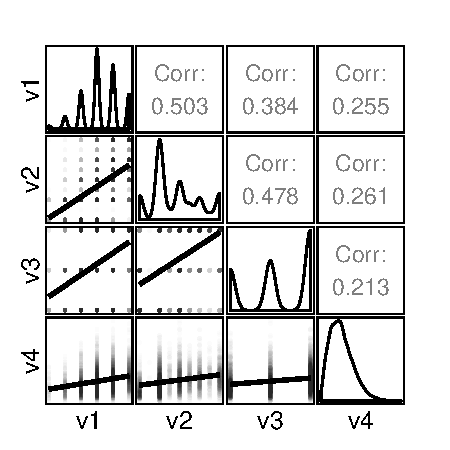
\includegraphics{../fig/corplot.pdf}
\caption{Correlation matrix of conventional political knowledge metrics and the text-based sophistication measure. The plots on the diagonal display unvariate densities for each variable. The panles in the lower triangular display the scatterplot of two measures as well as a linear fit. The upper triangular displays the correlation coefficient. All correlations reported are statistically significant with $p<.05$.}\label{fig:corplot}
\end{figure}


They are correlated but they are certainly not perfectly correlated. So is this variance meaningful? See below... The table displays responses with minimum and maximum composite scores for a subset of the data where the response was between 50 and 100 words. This initial investigation suggests that the variation in the sophistication measure captures interesting differences in response behavior that clearly overlaps with traditional knowledge metrics while displaying some unique variation.

\begin{table}[ht]\footnotesize\centering
\begin{tabular}{l|p{6.5cm}|p{6.5cm}}
   \toprule
  & Low Sophistication Response & High Sophistication Response \\ 
   \midrule
   Obama (+) & The healthcare, keeping that and the financial aid, helping students. & I think he is honest, has good intentions. \\ \hdashline
     Obama (-) &  & I don't feel he is up for the job, he doesn't really know how to get things accomplished from idea to actual reality. \\ \hdashline
     Romney (+) &  & He comes across as an honest person and I feel that financially he would be better for the country. \\ \hdashline
     Romney (-) & By taking financial aid away from students, taking family type planing, healthcare type of help away. & I am a moderate conservative and there are some things about anti-gay rights that I don't support. \\ \hdashline
     Democrats (+) & Mostly the healthcare, mostly people do need healthcare and can't afford to pay insurance. Financial aid most people cant afford to go college. Main two things that I like is the help with education and to pay for insurance to go to doctor. & They do seem to be generally concerned with everyone, taking care of the country as a whole. \\ \hdashline
     Democrats (-) &  & They fight too much among themselves and I disagree with wealth redistribution. \\ \hdashline
     Republicans (+) &  & I agree with a lot of the conservative values and taking responsibility for one's own actions. \\ \hdashline
     Republicans (-) &  & They argue too much among themselves and don't accomplish very much. \\ 
    \bottomrule
 \end{tabular}
\caption{Example of open-ended responses for low and high scores on the text-based sophistication measure with equal factual knowledge scores (3 out of 5 correct responses). The left column displays the verbatim responses of an individual who scored low on the text-based sophistication measure and the right column displays the verbatim responses of an individual who scored high on the text-based sophistication measure. Each row represents one of the likes/dislikes items included in the analysis. Note that the responses in this table were slightly redacted for readability (spelling errors removed, etc.).}\label{tab:ex1}
\end{table}

Political sophistication is not only of theoretical interest as a dependent variable in political science research, but commonly used as a determinant of other outcomes related to attitudes and behavior. Figure~\ref{fig:knoweff} presents the effects of each sophistication measure for men and women on four dependent variables commonly related to political sophistication: internal efficacy, external efficacy, non-conventional participation, and turnout. The results for the first three dependent variables are based on linear regressions while the effects on turnout are estimated using a logit model. Independent variables are the sophistication (interacted with gender) while controlling for age, race, religiosity, and survey mode (face-to-face vs. online). Each plot displays the expected value of the respective dependent variable (y-axis) for varying levels of each sophistication measure (x-axis), while holding all other variables at their respective means.

\begin{figure}[h]\centering
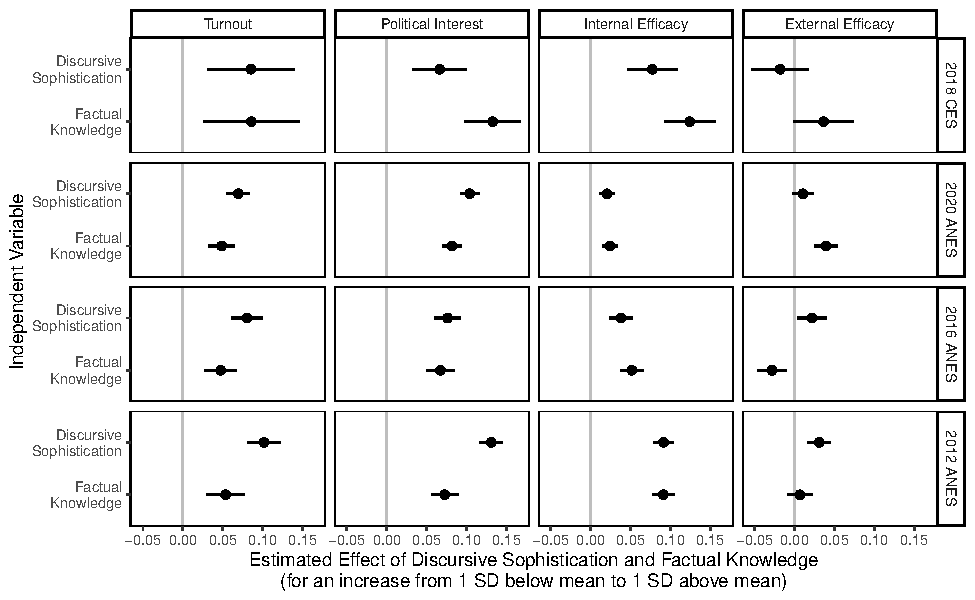
\includegraphics{../fig/knoweff.pdf}
\caption{Effects of sophistication on internal efficacy, external efficacy, non-conventional participation, and turnout. For each dependent variable, the figure displays the difference in expected values between maximum and minimum levels of sophistication observed on each measure (including 95\% confidence intervals). Model estimates are based on OLS (internal efficacy, external efficacy, non-conventional participation) or logistic regressions (turnout). Each sophistication measure is included in a single equation while controlling for gender, education, age, race, church attendance, and survey mode. Full model results ar presented in the appendix, Tables \ref{tab:inteff} through \ref{tab:turnout}}\label{fig:knoweff}
\end{figure}

Overall, the text-based measure performs at least as well as a predictor of internal efficacy, non-conventional participation, and turnout as the remaining variables. For some outcomes, the effect of text-based sophistication is even stronger than any of the conventional metrics. Furthermore, the effects of the text-based sophistication measure are constant across men and women. On the other hand, using factual knowledge, office recognition, or majorities in Congress, it appears that higher knowledge creates an apparent gender-gap in internal efficacy. Again, such a finding seems implausible, but could be explained by the fact that the traditional knowledge measures underestimate sophistication among women.



\section*{Are Women Really Less Sophisticated?}
% APPENDIX: add additional analyses controlling for wordsum score, substantive results are unchanged

How do men and women compare on the different metrics of political sophistication. Figure~\ref{fig:meandiff} displays the average levels of the text-based sophistication measure as well as the three conventional metrics comparing both genders.

\begin{figure}[h]\centering
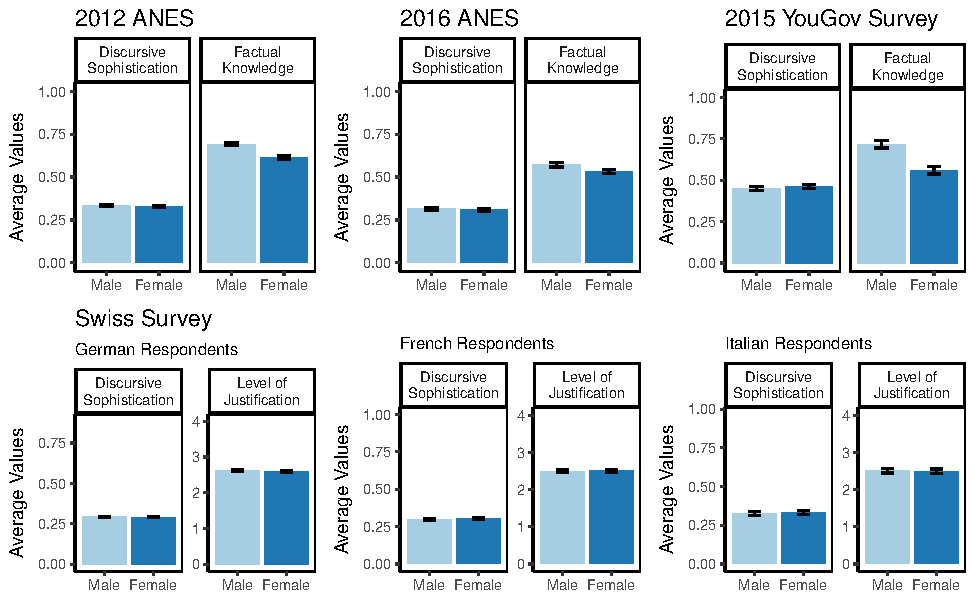
\includegraphics{../fig/meandiff.pdf}
\caption{The gender gap in political sophistication. The figure displays mean levels of sophistication for each measure comparing men and women (including 95\% confidence intervals). The y-axis is scaled to range up to the maximum value observed in the data for each sophistication metric. All gender differences are statistically significant with $p<.05$.}\label{fig:meandiff}
\end{figure}

While we observe a sizeable gender gap for all three conventional political knowledge measures, the difference is substantially smaller for the text-based sophistication measure. However, it could be argued that the gender gap can be attributed to real differences in resources such as education. As such, we now compare the gender gap while controlling for common determinants of political knowledge across all available measures. Beyond the gender gap, previous studies consistently showed that political knowledge is positively affected by media exposure, frequent political discussions, and education. Furthermore, the analyses includes several control variables such as age, race, religiosity, and survey mode (face-to-face vs. online). Figure~\ref{fig:determinants} displays the coefficients of regression models with each knowledge/sophistication measure as the dependent variable.

\begin{figure}[h]\centering
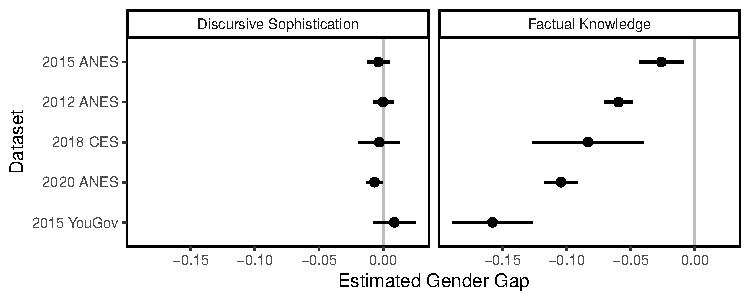
\includegraphics{../fig/determinants.pdf}
\caption{Common determinants of political sophistication. Estimates are OLS regression coefficients with 95\% confidence intervals. Dependent variables are the text-based sophistication measure as well as conventional metrics of political knowledge. Full model results are presented in the appendix, Table~\ref{tab:determinants}}\label{fig:determinants}
\end{figure}

Most importantly, while we still observe the gender gap using factual knowledge questions -- even after controlling for common determinants of sophistication -- the measure based on open-ended responses shows no significant differences. Women might not score as high on political information quizzes (partly because they are less likely to guess rather express lack of knowledge), but they do not differ substantially in complexity and sophistication when they describe their political preferences. The patterns for the remaining determinants are quite similar across different dependent variables. Knowledge and sophistication is significantly higher among respondents who are more exposed to political news media, discuss politics frequently, and are more educated. An interesting deviation, however, is the effect of survey mode. For factual knowledge questions, we observe that respondents in online surveys score significantly higher than individuals in face-to-face interviews. This difference could be explained by the fact that individuals are able to look up responses to factual knowledge questions while taking an online survey \citep[see also][]{clifford2016cheating}. For the text-based measure, on the other hand, we see that individuals appear to score lower on sophistication in online surveys. Respondents in online surveys might therefore be less willing to elaborate on their attitudes. Overall, the fact that the determinants of political sophistication are very consistent across models lends additional validity to the text-based measure.

As an additional step, we can examine whether women and men benefit equally from media exposure and political discussion according to the distinct measures. I extend the models from Figure~\ref{fig:determinants} by including an interaction between gender and media exposure as well as gender and political discussion. Based on this model, Figure~\ref{fig:closing} displays the expected sophistication levels for men and women on the four alternative measures while increasing exposure and discussion from it's minimum and maximum (holding all other variables constant at their respective means).

\begin{figure}[h]\centering

\includegraphics{../fig/closing.pdf}
\caption{Closing the gender gap. The figure displays the expected values of text-based sophistication and factual knowledge for men and women depending on their respective levels of media exposure, political discussion, and education (including 95\% confidence intervals). Estimates are based on OLS including interactions between gender and each independent variable. All models additionally control for education, age, race, church attendance, and survey mode. Full model results are presented in the appendix, Table~\ref{tab:closing}.}\label{fig:closing}
\end{figure}

Media exposure and political discussions increase political sophistication among men and women -- irrespective of the specific measurement. However, there are important differences between the text-based measure and conventional indices. For the traditional indices, we observe that the gender gap does not decrease among for higher levels of media exposure or political discussion. Indeed, media exposure even appears to increase gender differences in factual knowledge (and to a lesser extent office recognition). Such a result seems implausible, especially since recent research indicated that increased information mitigates the gender gap \citep{jerit2017revisiting}. For the text-based sophistication measure, on the other hand, women benefit at least as much as men (if not more) from media exposure and political discussion. The finding that media exposure increases the gender gap in factual knowledge might therefore be an artifact due to the fact that the measure underestimates knowledge for women.
% JENN: not satisfying



\section*{Conclusion}
% lot's of potential extensions, think about standardizing the measure to make it more comparable across contexts

Previous research in political science and public opinion has raised multiple theoretical and methodological issues related to conventional political knowledge indices. The goal of this paper is to examine an alternative measure of political sophistication based on open-ended responses in surveys. It was argued that this measure is conceptually closer to theoretical approaches that emphasize the importance of the structure and complexity of belief systems rather than focusing on factual knowledge about institutions. The findings show that conventional knowledge indices and the text-based measure share a substantial amount of variance. However, they are far from being identical and capture different aspects of sophistication. Most importantly, using the text-based measure, we don't find evidence for a gender gap that has been commonly reported using factual knowledge scales. While further work on validation and the comparability of the measure across contexts and survey modes is necessary, measuring political sophistication based on open-ended responses has the potential to provide novel insights into the antecedents and consequences of political sophistication.


\clearpage\singlespacing\footnotesize
\bibliographystyle{/data/Dropbox/Uni/Lit/apsr2006}
\bibliography{/data/Dropbox/Uni/Lit/Literature}

\clearpage
\section*{Appendix A: Details on Open-ended Responses}
\renewcommand\thefigure{A.\arabic{figure}}
\renewcommand\thetable{A.\arabic{table}}
\setcounter{figure}{0}
\setcounter{table}{0}

\begin{figure}[h]\centering
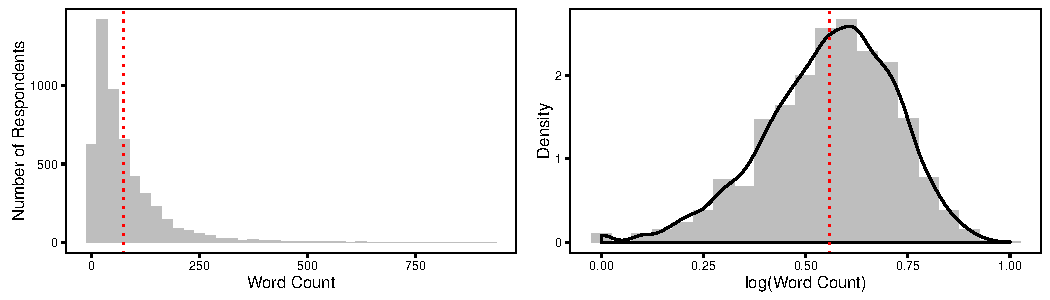
\includegraphics{../fig/wc.pdf}
\caption{Histogram of total word count in the collection of open-ended responses for each individual (left panel) and distribution of logged word count used in the text-based sophistication measure (right panel, re-scaled to range from 0 to 1). Dashed red lines indicate mean values. Most respondents provide brief statements when they describe their attitudes towards political parties and candidates. The mean response length to all 8 questions is about 75 words, so an average response to a single question consisted of less than 10 words, omitting respondents who did not provide any information.}\label{fig:wc}
\end{figure}

\begin{figure}[h]\centering
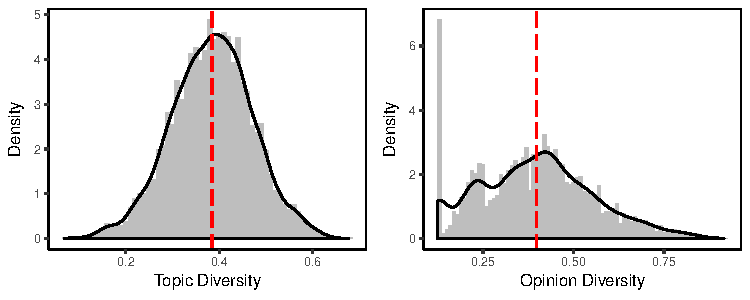
\includegraphics{../fig/diversity.pdf}
\caption{Histogram and density of the topic diversity (left panel) and opinion diversity (right panel) measure. Dashed red lines indicate mean values. The spike at 0 for opinion diversity are due to the fact that a large proportion of respondents only answered a single open-ended question.}\label{fig:diversity}
\end{figure}


\clearpage
\section*{Appendix B: Tables of Model Estimates}
\renewcommand\thefigure{B.\arabic{figure}}
\renewcommand\thetable{B.\arabic{table}}
\setcounter{figure}{0}
\setcounter{table}{0}


% Table created by stargazer v.5.2 by Marek Hlavac, Harvard University. E-mail: hlavac at fas.harvard.edu
% Date and time: Fri, Mar 31, 2017 - 11:40:40 PM
% Requires LaTeX packages: dcolumn 
\begin{table}[ht] \centering 
  \caption{Effects on Internal Efficacy} 
  \label{tab:inteff} 
\scriptsize 
\begin{tabular}{@{\extracolsep{-5pt}}lD{.}{.}{-3} D{.}{.}{-3} D{.}{.}{-3} D{.}{.}{-3} D{.}{.}{-3} D{.}{.}{-3} } 
\\[-1.8ex]\hline 
\hline \\[-1.8ex] 
 & \multicolumn{6}{c}{\textit{Dependent variable:}} \\ 
\cline{2-7} 
\\[-1.8ex] & \multicolumn{6}{c}{Iternal Efficacy} \\ 
\\[-1.8ex] & \multicolumn{1}{c}{(1)} & \multicolumn{1}{c}{(2)} & \multicolumn{1}{c}{(3)} & \multicolumn{1}{c}{(4)} & \multicolumn{1}{c}{(5)} & \multicolumn{1}{c}{(6)}\\ 
\hline \\[-1.8ex] 
 Text-based & 0.554^{***} &  &  &  &  &  \\ 
  & (0.035) &  &  &  &  &  \\ 
  Factual &  & 0.237^{***} &  &  &  &  \\ 
  &  & (0.015) &  &  &  &  \\ 
  Office &  &  & 0.248^{***} &  &  &  \\ 
  &  &  & (0.011) &  &  &  \\ 
  Majorities &  &  &  & 0.140^{***} &  &  \\ 
  &  &  &  & (0.008) &  &  \\ 
  Eval. (Pre) &  &  &  &  & 0.361^{***} &  \\ 
  &  &  &  &  & (0.019) &  \\ 
  Eval. (Post) &  &  &  &  &  & 0.285^{***} \\ 
  &  &  &  &  &  & (0.020) \\ 
  Sex (Female) & -0.062^{***} & -0.050^{***} & -0.052^{***} & -0.053^{***} & -0.038^{***} & -0.040^{***} \\ 
  & (0.006) & (0.006) & (0.006) & (0.006) & (0.010) & (0.010) \\ 
  Education (College) & 0.056^{***} & 0.055^{***} & 0.038^{***} & 0.063^{***} & 0.035^{**} & 0.044^{***} \\ 
  & (0.006) & (0.006) & (0.007) & (0.006) & (0.011) & (0.012) \\ 
  log(Age) & 0.019^{*} & 0.008 & 0.009 & 0.010 & -0.016 & -0.005 \\ 
  & (0.008) & (0.008) & (0.008) & (0.008) & (0.012) & (0.013) \\ 
  Race (Black) & 0.041^{***} & 0.058^{***} & 0.048^{***} & 0.042^{***} & 0.050^{***} & 0.059^{***} \\ 
  & (0.008) & (0.008) & (0.008) & (0.008) & (0.011) & (0.011) \\ 
  Church Attendance & 0.005 & 0.008 & 0.013 & 0.005 & -0.003 & -0.009 \\ 
  & (0.008) & (0.008) & (0.008) & (0.009) & (0.014) & (0.015) \\ 
  Survey Mode (Online) & 0.047^{***} & 0.009 & -0.009 & 0.001 &  &  \\ 
  & (0.006) & (0.006) & (0.007) & (0.007) &  &  \\ 
  Constant & 0.179^{***} & 0.368^{***} & 0.442^{***} & 0.444^{***} & 0.377^{***} & 0.400^{***} \\ 
  & (0.033) & (0.030) & (0.030) & (0.031) & (0.044) & (0.047) \\ 
 \hline \\[-1.8ex] 
Observations & \multicolumn{1}{c}{5,135} & \multicolumn{1}{c}{5,135} & \multicolumn{1}{c}{4,816} & \multicolumn{1}{c}{4,816} & \multicolumn{1}{c}{1,743} & \multicolumn{1}{c}{1,647} \\ 
R$^{2}$ & \multicolumn{1}{c}{0.114} & \multicolumn{1}{c}{0.116} & \multicolumn{1}{c}{0.160} & \multicolumn{1}{c}{0.128} & \multicolumn{1}{c}{0.228} & \multicolumn{1}{c}{0.170} \\ 
\hline 
\hline \\[-1.8ex] 
\textit{Note:}  & \multicolumn{6}{r}{$^{*}$p$<$0.05; $^{**}$p$<$0.01; $^{***}$p$<$0.001} \\ 
\end{tabular} 
\end{table} 


% Table created by stargazer v.5.2 by Marek Hlavac, Harvard University. E-mail: hlavac at fas.harvard.edu
% Date and time: Thu, Jun 22, 2017 - 04:21:44 PM
% Requires LaTeX packages: dcolumn 
\begin{table}[ht] \centering 
  \caption{Effects of sophistication -- OLS models predicting external efficacy 
          based on different sophistication 
          measures. Positive coefficients indicate higher self-reported external efficacy. 
          Standard errors in parentheses. Estimates are used for Figure~\ref{fig:knoweff} 
          in the main text.} 
  \label{tab:exteff} 
\scriptsize 
\begin{tabular}{@{\extracolsep{-5pt}}lD{.}{.}{-3} D{.}{.}{-3} D{.}{.}{-3} D{.}{.}{-3} D{.}{.}{-3} D{.}{.}{-3} } 
\\[-1.8ex]\hline 
\hline \\[-1.8ex] 
 & \multicolumn{6}{c}{\textit{Dependent variable:}} \\ 
\cline{2-7} 
\\[-1.8ex] & \multicolumn{6}{c}{External Efficacy} \\ 
\hline \\[-1.8ex] 
 Text-based & 0.110^{**} &  &  &  &  &  \\ 
  & (0.041) &  &  &  &  &  \\ 
  Factual &  & 0.049^{**} &  &  &  &  \\ 
  &  & (0.017) &  &  &  &  \\ 
  Office &  &  & 0.084^{***} &  &  &  \\ 
  &  &  & (0.013) &  &  &  \\ 
  Majorities &  &  &  & 0.044^{***} &  &  \\ 
  &  &  &  & (0.010) &  &  \\ 
  Eval. (Pre) &  &  &  &  & 0.136^{***} &  \\ 
  &  &  &  &  & (0.026) &  \\ 
  Eval. (Post) &  &  &  &  &  & 0.149^{***} \\ 
  &  &  &  &  &  & (0.027) \\ 
  Sex (Female) & 0.014^{*} & 0.016^{*} & 0.015^{*} & 0.015^{*} & 0.023 & 0.023 \\ 
  & (0.007) & (0.007) & (0.007) & (0.007) & (0.013) & (0.014) \\ 
  Education (College) & 0.041^{***} & 0.041^{***} & 0.033^{***} & 0.040^{***} & 0.064^{***} & 0.057^{***} \\ 
  & (0.008) & (0.008) & (0.008) & (0.008) & (0.016) & (0.016) \\ 
  Income & 0.023 & 0.021 & 0.012 & 0.021 & 0.006 & 0.002 \\ 
  & (0.012) & (0.012) & (0.013) & (0.013) & (0.025) & (0.025) \\ 
  log(Age) & -0.008 & -0.011 & -0.013 & -0.012 & -0.051^{**} & -0.048^{**} \\ 
  & (0.009) & (0.009) & (0.010) & (0.010) & (0.016) & (0.017) \\ 
  Race (Black) & 0.077^{***} & 0.080^{***} & 0.078^{***} & 0.076^{***} & 0.058^{***} & 0.058^{***} \\ 
  & (0.009) & (0.009) & (0.009) & (0.009) & (0.015) & (0.015) \\ 
  Church Attendance & 0.048^{***} & 0.049^{***} & 0.053^{***} & 0.050^{***} & 0.045^{*} & 0.042^{*} \\ 
  & (0.010) & (0.010) & (0.010) & (0.010) & (0.019) & (0.020) \\ 
  Survey Mode (Online) & -0.036^{***} & -0.043^{***} & -0.055^{***} & -0.051^{***} &  &  \\ 
  & (0.008) & (0.008) & (0.008) & (0.008) &  &  \\ 
  Constant & 0.369^{***} & 0.407^{***} & 0.434^{***} & 0.432^{***} & 0.462^{***} & 0.455^{***} \\ 
  & (0.038) & (0.035) & (0.036) & (0.037) & (0.061) & (0.063) \\ 
 \hline \\[-1.8ex] 
Observations & \multicolumn{1}{c}{4,993} & \multicolumn{1}{c}{4,993} & \multicolumn{1}{c}{4,694} & \multicolumn{1}{c}{4,694} & \multicolumn{1}{c}{1,653} & \multicolumn{1}{c}{1,569} \\ 
R$^{2}$ & \multicolumn{1}{c}{0.040} & \multicolumn{1}{c}{0.040} & \multicolumn{1}{c}{0.048} & \multicolumn{1}{c}{0.044} & \multicolumn{1}{c}{0.053} & \multicolumn{1}{c}{0.053} \\ 
\hline 
\hline \\[-1.8ex] 
\textit{Note:}  & \multicolumn{6}{r}{$^{*}$p$<$0.05; $^{**}$p$<$0.01; $^{***}$p$<$0.001} \\ 
\end{tabular} 
\end{table} 


% Table created by stargazer v.5.2 by Marek Hlavac, Harvard University. E-mail: hlavac at fas.harvard.edu
% Date and time: Mon, Apr 03, 2017 - 04:16:07 PM
% Requires LaTeX packages: dcolumn 
\begin{table}[ht] \centering 
  \caption{Effects of sophistication -- OLS models predicting non-conventional 
          particpation (protest, signing 
          petitions, etc.) based on different sophistication 
          measures. Positive coefficients indicate higher levels of participation. 
          Standard errors in parentheses. Estimates are used for Figure~\ref{fig:knoweff} 
          in the main text.} 
  \label{tab:nonconv} 
\scriptsize 
\begin{tabular}{@{\extracolsep{-5pt}}lD{.}{.}{-3} D{.}{.}{-3} D{.}{.}{-3} D{.}{.}{-3} D{.}{.}{-3} D{.}{.}{-3} } 
\\[-1.8ex]\hline 
\hline \\[-1.8ex] 
 & \multicolumn{6}{c}{\textit{Dependent variable:}} \\ 
\cline{2-7} 
\\[-1.8ex] & \multicolumn{6}{c}{Non-conventional Participation} \\ 
\hline \\[-1.8ex] 
 Text-based & 1.150^{***} &  &  &  &  &  \\ 
  & (0.084) &  &  &  &  &  \\ 
  Factual &  & 0.212^{***} &  &  &  &  \\ 
  &  & (0.036) &  &  &  &  \\ 
  Office &  &  & 0.331^{***} &  &  &  \\ 
  &  &  & (0.027) &  &  &  \\ 
  Majorities &  &  &  & 0.159^{***} &  &  \\ 
  &  &  &  & (0.019) &  &  \\ 
  Eval. (Pre) &  &  &  &  & 0.452^{***} &  \\ 
  &  &  &  &  & (0.048) &  \\ 
  Eval. (Post) &  &  &  &  &  & 0.445^{***} \\ 
  &  &  &  &  &  & (0.048) \\ 
  Sex (Female) & 0.007 & 0.014 & 0.022 & 0.017 & 0.025 & 0.027 \\ 
  & (0.014) & (0.014) & (0.014) & (0.014) & (0.024) & (0.024) \\ 
  Education (College) & 0.089^{***} & 0.122^{***} & 0.088^{***} & 0.125^{***} & 0.103^{***} & 0.099^{***} \\ 
  & (0.016) & (0.016) & (0.016) & (0.015) & (0.028) & (0.028) \\ 
  log(Age) & 0.035 & 0.040^{*} & 0.027 & 0.033 & -0.052 & -0.047 \\ 
  & (0.019) & (0.020) & (0.019) & (0.019) & (0.030) & (0.030) \\ 
  Race (Black) & 0.036 & 0.044^{*} & 0.040^{*} & 0.030 & -0.020 & -0.011 \\ 
  & (0.018) & (0.019) & (0.019) & (0.019) & (0.027) & (0.027) \\ 
  Church Attendance & 0.028 & 0.035 & 0.041^{*} & 0.031 & 0.047 & 0.041 \\ 
  & (0.020) & (0.020) & (0.020) & (0.020) & (0.035) & (0.035) \\ 
  Survey Mode (Online) & 0.103^{***} & 0.051^{**} & 0.019 & 0.039^{*} &  &  \\ 
  & (0.015) & (0.016) & (0.016) & (0.016) &  &  \\ 
  Constant & -0.392^{***} & 0.032 & 0.130 & 0.121 & 0.275^{*} & 0.287^{*} \\ 
  & (0.080) & (0.074) & (0.073) & (0.074) & (0.112) & (0.112) \\ 
 \hline \\[-1.8ex] 
Observations & \multicolumn{1}{c}{4,809} & \multicolumn{1}{c}{4,809} & \multicolumn{1}{c}{4,809} & \multicolumn{1}{c}{4,809} & \multicolumn{1}{c}{1,638} & \multicolumn{1}{c}{1,638} \\ 
R$^{2}$ & \multicolumn{1}{c}{0.068} & \multicolumn{1}{c}{0.038} & \multicolumn{1}{c}{0.061} & \multicolumn{1}{c}{0.045} & \multicolumn{1}{c}{0.078} & \multicolumn{1}{c}{0.075} \\ 
\hline 
\hline \\[-1.8ex] 
\textit{Note:}  & \multicolumn{6}{r}{$^{*}$p$<$0.05; $^{**}$p$<$0.01; $^{***}$p$<$0.001} \\ 
\end{tabular} 
\end{table} 


% Table created by stargazer v.5.2 by Marek Hlavac, Harvard University. E-mail: hlavac at fas.harvard.edu
% Date and time: Fri, Mar 31, 2017 - 11:40:45 PM
% Requires LaTeX packages: dcolumn 
\begin{table}[ht] \centering 
  \caption{Effects on Turnout (Logit)} 
  \label{tab:turnout} 
\scriptsize 
\begin{tabular}{@{\extracolsep{-5pt}}lD{.}{.}{-3} D{.}{.}{-3} D{.}{.}{-3} D{.}{.}{-3} D{.}{.}{-3} D{.}{.}{-3} } 
\\[-1.8ex]\hline 
\hline \\[-1.8ex] 
 & \multicolumn{6}{c}{\textit{Dependent variable:}} \\ 
\cline{2-7} 
\\[-1.8ex] & \multicolumn{6}{c}{Turnout} \\ 
\hline \\[-1.8ex] 
 Text-based & 5.521^{***} &  &  &  &  &  \\ 
  & (0.487) &  &  &  &  &  \\ 
  Factual &  & 1.376^{***} &  &  &  &  \\ 
  &  & (0.197) &  &  &  &  \\ 
  Office &  &  & 2.213^{***} &  &  &  \\ 
  &  &  & (0.180) &  &  &  \\ 
  Majorities &  &  &  & 1.152^{***} &  &  \\ 
  &  &  &  & (0.108) &  &  \\ 
  Eval. (Pre) &  &  &  &  & 2.942^{***} &  \\ 
  &  &  &  &  & (0.271) &  \\ 
  Eval. (Post) &  &  &  &  &  & 2.831^{***} \\ 
  &  &  &  &  &  & (0.276) \\ 
  Sex (Female) & 0.045 & 0.054 & 0.120 & 0.112 & 0.143 & 0.145 \\ 
  & (0.082) & (0.081) & (0.083) & (0.082) & (0.130) & (0.130) \\ 
  Education (College) & 0.699^{***} & 0.804^{***} & 0.615^{***} & 0.815^{***} & 0.723^{***} & 0.679^{***} \\ 
  & (0.104) & (0.103) & (0.105) & (0.102) & (0.177) & (0.176) \\ 
  log(Age) & 1.086^{***} & 1.061^{***} & 0.993^{***} & 1.011^{***} & 0.773^{***} & 0.759^{***} \\ 
  & (0.102) & (0.102) & (0.103) & (0.103) & (0.156) & (0.156) \\ 
  Race (Black) & 0.649^{***} & 0.728^{***} & 0.682^{***} & 0.629^{***} & 0.772^{***} & 0.808^{***} \\ 
  & (0.115) & (0.116) & (0.114) & (0.114) & (0.157) & (0.156) \\ 
  Church Attendance & 0.717^{***} & 0.738^{***} & 0.767^{***} & 0.721^{***} & 0.830^{***} & 0.753^{***} \\ 
  & (0.125) & (0.124) & (0.125) & (0.125) & (0.199) & (0.198) \\ 
  Survey Mode (Online) & 0.719^{***} & 0.412^{***} & 0.234^{**} & 0.281^{**} &  &  \\ 
  & (0.086) & (0.086) & (0.087) & (0.088) &  &  \\ 
  Constant & -6.628^{***} & -4.563^{***} & -4.002^{***} & -3.947^{***} & -4.101^{***} & -3.800^{***} \\ 
  & (0.440) & (0.384) & (0.388) & (0.387) & (0.587) & (0.579) \\ 
 \hline \\[-1.8ex] 
Observations & \multicolumn{1}{c}{4,831} & \multicolumn{1}{c}{4,831} & \multicolumn{1}{c}{4,812} & \multicolumn{1}{c}{4,812} & \multicolumn{1}{c}{1,647} & \multicolumn{1}{c}{1,645} \\ 
Akaike Inf. Crit. & \multicolumn{1}{c}{3,937.628} & \multicolumn{1}{c}{4,022.502} & \multicolumn{1}{c}{3,893.755} & \multicolumn{1}{c}{3,948.129} & \multicolumn{1}{c}{1,550.512} & \multicolumn{1}{c}{1,563.228} \\ 
\hline 
\hline \\[-1.8ex] 
\textit{Note:}  & \multicolumn{6}{r}{$^{*}$p$<$0.05; $^{**}$p$<$0.01; $^{***}$p$<$0.001} \\ 
\end{tabular} 
\end{table} 


% Table created by stargazer v.5.2 by Marek Hlavac, Harvard University. E-mail: hlavac at fas.harvard.edu
% Date and time: Wed, Jun 14, 2017 - 11:02:19 AM
% Requires LaTeX packages: dcolumn 
\begin{table}[ht] \centering 
  \caption{Determinants of political knowledge -- OLS models predicting different 
          political sophistication measures.
          Positive coefficients indicate higher sophistication. 
          Standard errors in parentheses. Estimates are used for Figure~\ref{fig:determinants} 
          in the main text.} 
  \label{tab:determinants} 
\scriptsize 
\begin{tabular}{@{\extracolsep{-5pt}}lD{.}{.}{-3} D{.}{.}{-3} D{.}{.}{-3} D{.}{.}{-3} D{.}{.}{-3} D{.}{.}{-3} } 
\\[-1.8ex]\hline 
\hline \\[-1.8ex] 
 & \multicolumn{6}{c}{Dependent Variable: Political Knowledge Measure} \\ 
\cline{2-7} 
\\[-1.8ex] & \multicolumn{1}{c}{Text-based} & \multicolumn{1}{c}{Factual} & \multicolumn{1}{c}{Office} & \multicolumn{1}{c}{Majorities} & \multicolumn{1}{c}{Eval. (Pre)} & \multicolumn{1}{c}{Eval. (Post)} \\ 
\hline \\[-1.8ex] 
 Gender (Female) & -0.002 & -0.049^{***} & -0.045^{***} & -0.082^{***} & -0.046^{***} & -0.052^{***} \\ 
  & (0.002) & (0.006) & (0.007) & (0.011) & (0.012) & (0.012) \\ 
  Media Exposure & 0.024^{***} & 0.069^{***} & 0.159^{***} & 0.193^{***} & 0.255^{***} & 0.192^{***} \\ 
  & (0.006) & (0.014) & (0.018) & (0.026) & (0.030) & (0.030) \\ 
  Political Discussions & 0.056^{***} & 0.062^{***} & 0.195^{***} & 0.200^{***} & 0.144^{***} & 0.174^{***} \\ 
  & (0.004) & (0.010) & (0.013) & (0.019) & (0.019) & (0.019) \\ 
  Education (College) & 0.038^{***} & 0.091^{***} & 0.129^{***} & 0.099^{***} & 0.100^{***} & 0.118^{***} \\ 
  & (0.003) & (0.007) & (0.008) & (0.012) & (0.014) & (0.014) \\ 
  Income & 0.031^{***} & 0.117^{***} & 0.147^{***} & 0.091^{***} & 0.142^{***} & 0.135^{***} \\ 
  & (0.004) & (0.010) & (0.013) & (0.019) & (0.022) & (0.022) \\ 
  log(Age) & 0.012^{***} & 0.081^{***} & 0.048^{***} & 0.122^{***} & 0.057^{***} & 0.062^{***} \\ 
  & (0.003) & (0.008) & (0.010) & (0.015) & (0.015) & (0.015) \\ 
  Race (Black) & -0.009^{**} & -0.085^{***} & -0.036^{***} & -0.034^{*} & 0.031^{*} & 0.020 \\ 
  & (0.003) & (0.008) & (0.010) & (0.014) & (0.014) & (0.014) \\ 
  Church Attendance & 0.004 & -0.004 & -0.028^{**} & 0.014 & 0.003 & 0.014 \\ 
  & (0.003) & (0.008) & (0.010) & (0.015) & (0.017) & (0.017) \\ 
  Survey Mode (Online) & -0.024^{***} & 0.093^{***} & 0.163^{***} & 0.214^{***} &  &  \\ 
  & (0.003) & (0.006) & (0.008) & (0.012) &  &  \\ 
  Constant & 0.389^{***} & 0.101^{***} & -0.198^{***} & -0.376^{***} & 0.199^{***} & 0.137^{*} \\ 
  & (0.012) & (0.030) & (0.038) & (0.055) & (0.056) & (0.055) \\ 
 \hline \\[-1.8ex] 
Observations & \multicolumn{1}{c}{4,698} & \multicolumn{1}{c}{4,698} & \multicolumn{1}{c}{4,698} & \multicolumn{1}{c}{4,698} & \multicolumn{1}{c}{1,575} & \multicolumn{1}{c}{1,575} \\ 
R$^{2}$ & \multicolumn{1}{c}{0.159} & \multicolumn{1}{c}{0.282} & \multicolumn{1}{c}{0.322} & \multicolumn{1}{c}{0.225} & \multicolumn{1}{c}{0.242} & \multicolumn{1}{c}{0.251} \\ 
\hline 
\hline \\[-1.8ex] 
\textit{Note:}  & \multicolumn{6}{r}{$^{*}$p$<$0.05; $^{**}$p$<$0.01; $^{***}$p$<$0.001} \\ 
\end{tabular} 
\end{table} 


% Table created by stargazer v.5.2 by Marek Hlavac, Harvard University. E-mail: hlavac at fas.harvard.edu
% Date and time: Wed, Jun 14, 2017 - 11:02:21 AM
% Requires LaTeX packages: dcolumn 
\begin{table}[ht] \centering 
  \caption{Closing the Gender Gap -- OLS models predicting different 
          political sophistication measures.
          Positive coefficients indicate higher sophistication. 
          Standard errors in parentheses. Estimates are used for 
          Figure~\ref{fig:closing} in the main text.} 
  \label{tab:closing} 
\scriptsize 
\begin{tabular}{@{\extracolsep{-5pt}}lD{.}{.}{-3} D{.}{.}{-3} } 
\\[-1.8ex]\hline 
\hline \\[-1.8ex] 
 & \multicolumn{2}{c}{Dependent Variable: Political Knowledge Measure} \\ 
\cline{2-3} 
\\[-1.8ex] & \multicolumn{1}{c}{Text-based} & \multicolumn{1}{c}{Factual} \\ 
\hline \\[-1.8ex] 
 Gender (Female) & -0.011^{*} & -0.016 \\ 
  & (0.005) & (0.013) \\ 
  Media Exposure & 0.017^{*} & 0.097^{***} \\ 
  & (0.008) & (0.020) \\ 
  Political Discussions & 0.055^{***} & 0.068^{***} \\ 
  & (0.006) & (0.014) \\ 
  Education (College) & 0.035^{***} & 0.098^{***} \\ 
  & (0.004) & (0.009) \\ 
  Income & 0.031^{***} & 0.117^{***} \\ 
  & (0.004) & (0.010) \\ 
  log(Age) & 0.012^{***} & 0.080^{***} \\ 
  & (0.003) & (0.008) \\ 
  Race (Black) & -0.009^{**} & -0.085^{***} \\ 
  & (0.003) & (0.008) \\ 
  Church Attendance & 0.004 & -0.004 \\ 
  & (0.003) & (0.008) \\ 
  Survey Mode (Online) & -0.024^{***} & 0.093^{***} \\ 
  & (0.003) & (0.006) \\ 
  Female * Media & 0.014 & -0.056^{*} \\ 
  & (0.011) & (0.026) \\ 
  Female * Discussions & 0.001 & -0.011 \\ 
  & (0.008) & (0.020) \\ 
  Female * Education & 0.007 & -0.016 \\ 
  & (0.005) & (0.012) \\ 
  Constant & 0.392^{***} & 0.087^{**} \\ 
  & (0.013) & (0.031) \\ 
 \hline \\[-1.8ex] 
Observations & \multicolumn{1}{c}{4,698} & \multicolumn{1}{c}{4,698} \\ 
R$^{2}$ & \multicolumn{1}{c}{0.160} & \multicolumn{1}{c}{0.284} \\ 
\hline 
\hline \\[-1.8ex] 
\textit{Note:}  & \multicolumn{2}{r}{$^{*}$p$<$0.05; $^{**}$p$<$0.01; $^{***}$p$<$0.001} \\ 
\end{tabular} 
\end{table} 


\end{document}